% !TEX root =./main.tex

\section{Block 5: Beamforming}
Author: Victor Chen

Beamforming is a signal processing technique used to spatially direct signals, enhancing desired signals while suppressing other signals with interference. A delay-and-sum beamforming algorithm is applied to the four-channel system of uniformly spaced linear sensor array of four omnidirectional microphones. Assuming the signal source is in the far field, the incoming wave fronts are approximately linear, enabling the computation of beam angle for each integer sample delay k.

The goal for the beamforming block is to use the delay-and-sum beamforming function 
\begin{align*}
    Beams[k,n] = X_1[n]+X_2[n+k]+X_3[n+2*k]+X+4[n+3*k]
\end{align*}
to spatially focus and enhance signals from a specific direction across our four-channel system.


\subsection{Implementation}

This block is designed to perform beamforming across 4,000 samples from the four channels. Given the need for multiple iterations, it is crucial to balance between processing speed and output quality.

To optimize the beamforming function, we utilize \textsc{MATLAB}'s linear vectorization and precomputing capabilities, enabling faster and more efficient processing by operating on entire data arrays simultaneously instead of relying solely on iterative loops.

\begin{figure}[H]
    \centering
    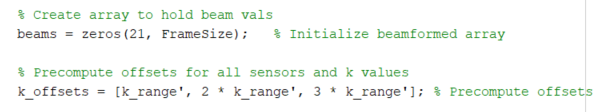
\includegraphics[width=0.5\linewidth]{figures/beamform_fig1.png}
    \caption{Precomuting Equations}
    \label{fig:precomputing_equations}
\end{figure}

The first optimization method involves precomputing the array to store the beams and the offsets for all sensors. This approach preloads the necessary matrices, eliminating the need for dynamic resizing or appending during runtime, which can significantly slow down the program. As illustrated in Figure 1, the k\_offsets for the delays are computed in a single step using vectorized operations. Additionally, a beams array is preallocated in advance to hold the calculated beams, ensuring optimal memory usage and faster processing.

\begin{figure}[H]
    \centering
    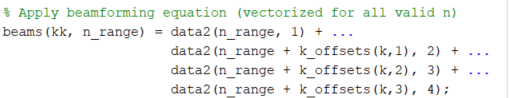
\includegraphics[width=0.5\linewidth]{figures/beamform_fig2.png}
    \caption{Beamforming Computation}
    \label{fig:beamforming_computation}
\end{figure}

The second optimization method involves performing beamforming calculations across all 4,000 samples simultaneously, rather than iterating through each index individually. This reduces the number of loops, making the process much more efficient.



\subsection{Analysis}

After developing the beamforming function, test data was generated to evaluate its performance. The test data consisted of four channels of in-phase sine waves, defined by the equation \textit{sample} = sin(\textit{t}/40), where \textit{t} ranged from 1 to 4,000. After ensuring the function works with the test data, I used data2 directly from the project.

\begin{figure}[H]
    \centering
    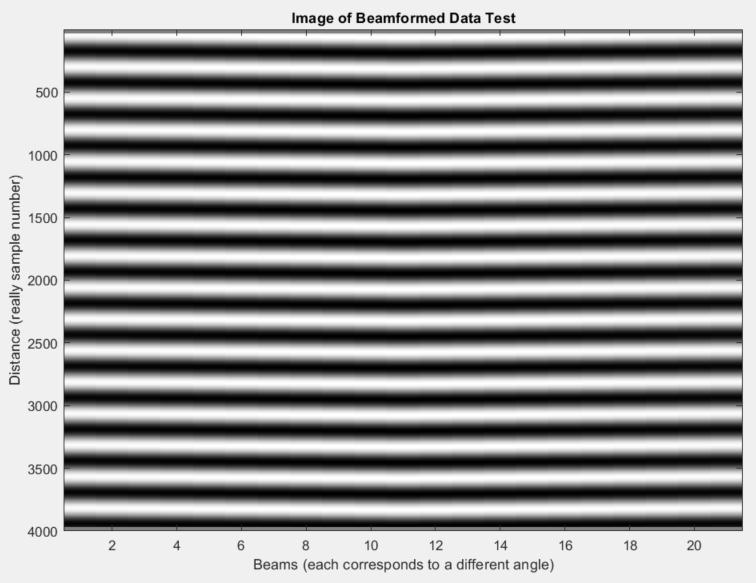
\includegraphics[width=0.5\linewidth]{figures/beamform_fig3.png}
    \caption{Output for Testing with sin(t/40) wave}
    \label{fig:sinwave_output}
\end{figure}

As shown in Figure 3, each black-and-white horizontal line represents a wave. With 4,000 samples in the equation sin(\textit{t}/40), this corresponds to approximately 16 waves. The figure confirms this, demonstrating that the beamforming function performs as expected. It is important to note that the waves are evenly horizontal due to the in-phase channels, however, as the frequency of the waves increases, the evenness of the waves will begin to separate.

\begin{figure}[H]
    \centering
    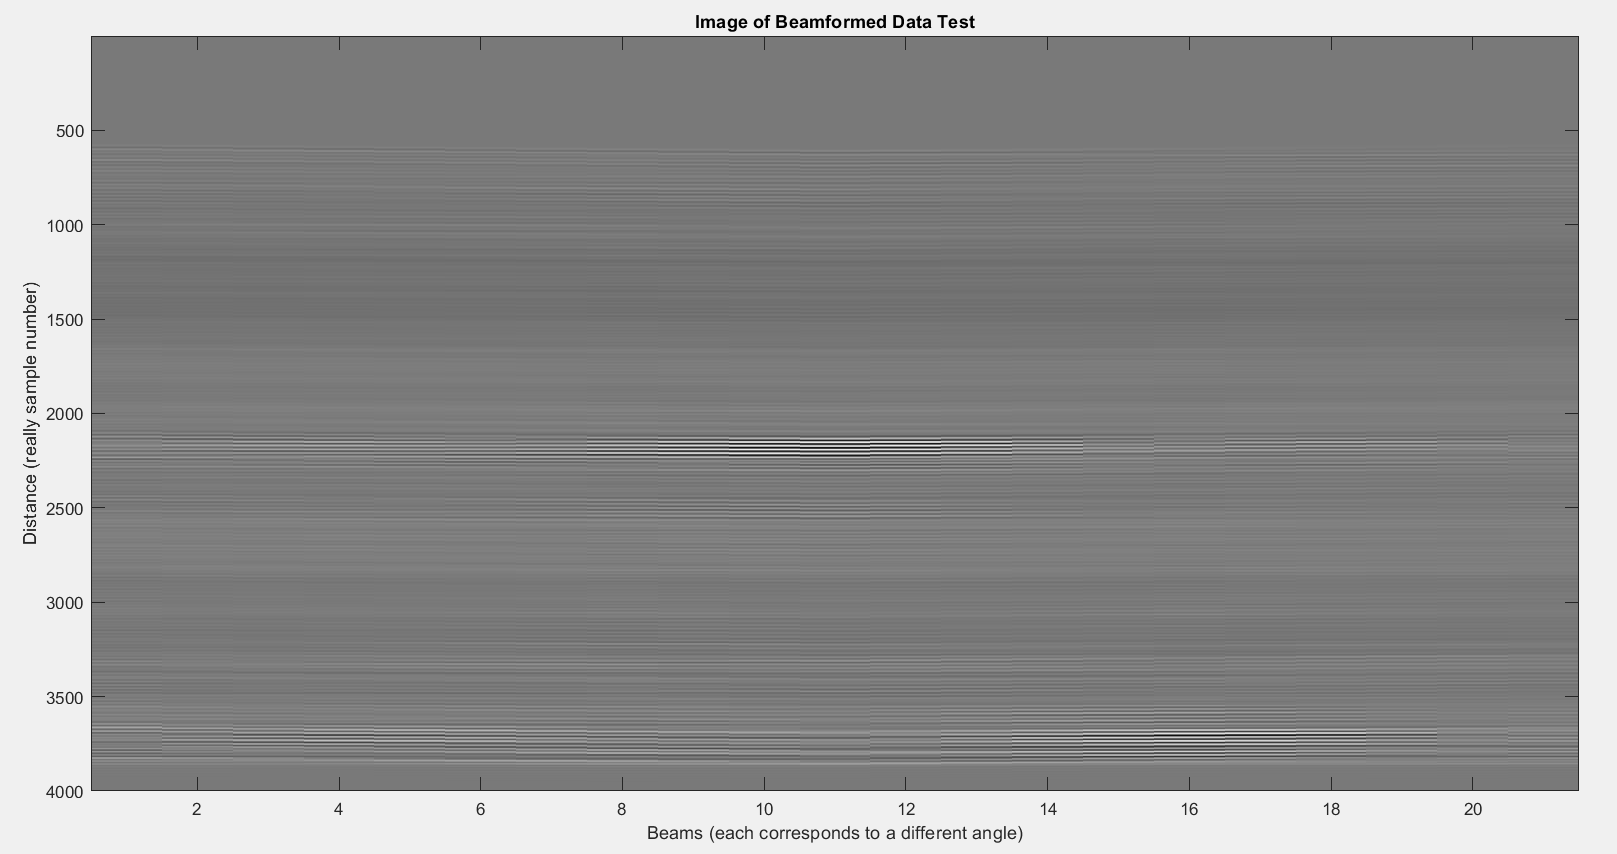
\includegraphics[width=0.5\linewidth]{figures/beamform_fig4.png}
    \caption{Beamform Output from Data}
    \label{fig:final_beamform_output}
\end{figure}

As shown in Figure 4, the beamform output of data2 reveals two regions where the signal strength is highest. These are represented by two prominent white "blobs"--one near the center and another near the bottom-right corner of the beamformed image. These regions indicate areas where the waves return well-constructed, suggesting the presence of an object that the waves interacted with.

\begin{figure}[H]
    \centering
    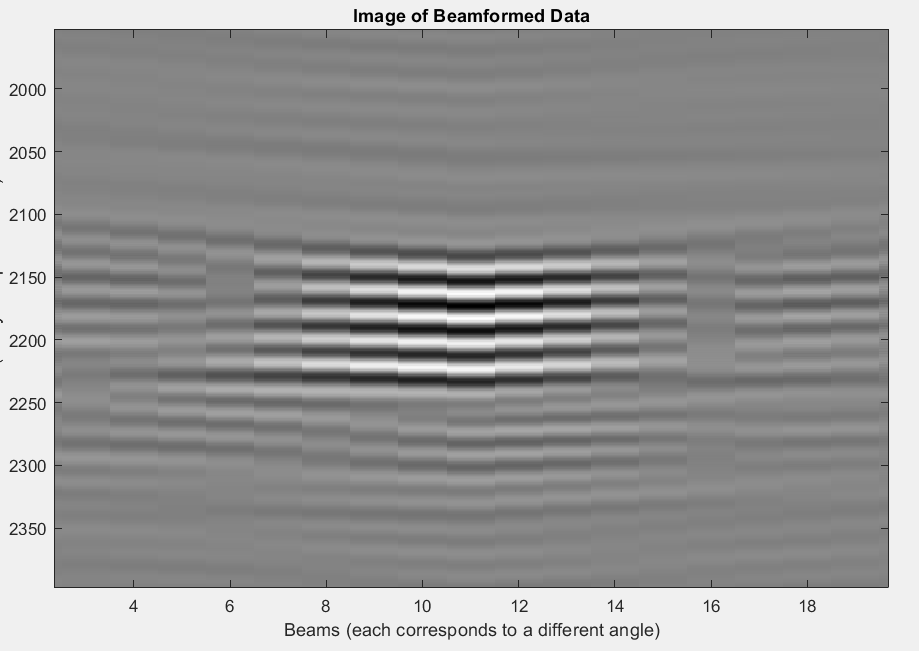
\includegraphics[width=0.5\linewidth]{figures/beamform_fig5.png}
    \caption{Zoomed In Beamform Output}
    \label{fig:zoomed_in_beamform_output}
\end{figure}

By zooming into the center of the beamform image in Figure 5, we can see that while the signal strength is high, each beam is still slightly offset. This offset may be due to inaccuracies in my delay calculations or it might be due to the geometry/spacing of the sensors. Plenty of time was spent on trying to correct the offset by shifting beams, however none were successful. More work will need to be done to correct this issue.


The beamforming function achieved an average execution time of 0.0023155 seconds, a substantial improvement compared to pre-optimization runs, which took tens of seconds. This demonstrates a significant increase in computational efficiency for beamforming.
